\subsubsection{Description (type, operation parameters)}
\iffalse Describe the IMD used and use a table for the common operation parameters, like supply voltage, set point, etc. Also, describe how the IMD indicator light is wired, etc.
Additionally, fill out the following table replacing the values with your specification:\fi

We use A-ISOMETER® IR155-3203 Insulation monitoring device (IMD) for unearthed DC drive systems. Our maximum tractive voltage is 403.2 VDC. The rules require minimal insulation value between TS and GLVS 500 Ohm/V. Minimal resistance value for our car is 403.2*500 = 201 600 Ohm. This was set as request for manufacturer, and device was programmed in factory.
\begin{table}[H]
	\centering
	\caption{Parameters of the IMD}
	\begin{tabularx}{\textwidth}{|X|l|}
	 \hline	Supply voltage range: & 10..36VDC \\[.4cm]
	 \hline	Supply voltage & 24VDC \\[.4cm]
	 \hline	Environmental temperature range: & -40..105°C \\[.4cm]
	 \hline	Selftest interval: & Always at startup, then every 5 minutes \\[.4cm]
	 \hline	High voltage range: & DC 0..1000V \\[.4cm]
	 \hline	Set response value: & 201.6kΩ (500Ω/Volt) \\[.4cm]
	 \hline	Max. operation current: & 150mA \\[.4cm]
	 \hline	Approximate time to shut down at 50\% of the response value: & 20s \\[.4cm]
	  \hline
	\end{tabularx}%
	\label{tab:IMD}%
\end{table}%

\subsubsection{Wiring/cables/connectors/}
 Describe wiring, show schematics, describe connectors and cables used and show useful data regarding the wiring including wire gauge/temp/voltage rating and fuses protecting the wiring. 

\iffalse Relay of Insulation Monitoring Device is electrically placed between relay in ECUB and relay for AMS measurement. Wiring is done using Raychem Spec44 wire, AWG 26, rated to 600V. Wiring is shown on \ref{label}. Fusing is shown at \ref{label}. IMD opens relay in case of fault. IMD have output for relay, so there is not necessary adding zero diode on output. HV input to IMD is connected in according to datasheet. \fi

\subsubsection{Position in car}
Provide CAD-renderings showing the relevant parts. Mark the parts in the rendering, if necessary

\begin{figure}[H]
	\centering
	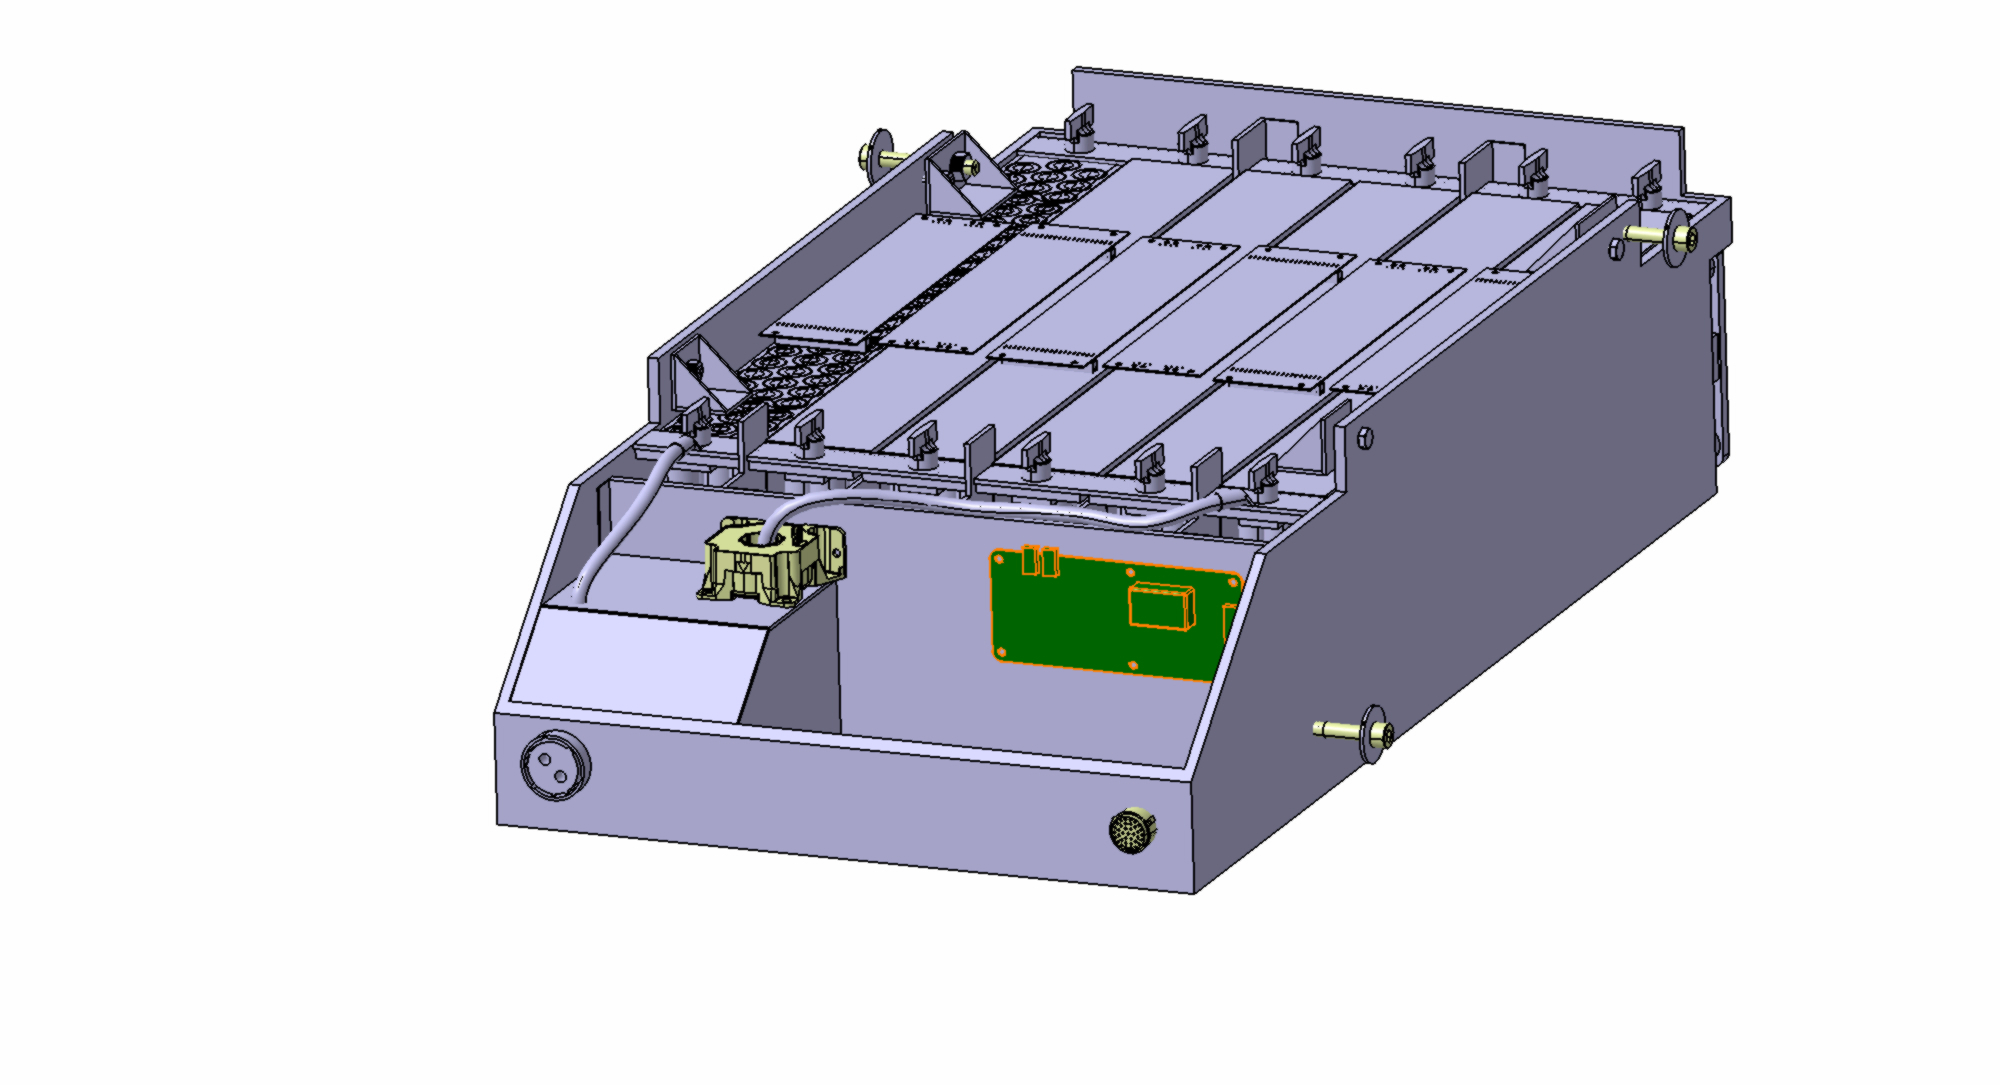
\includegraphics[width=\textwidth,trim={0cm 0cm 0cm 0cm},clip]{./img/IMD-position.jpg}
	\caption{IMD position.}
	\label{fig:IMD-position}
\end{figure}
